%chap 3
\chapter{بررسی پژوهش‌های پیشین}
\thispagestyle{empty}
\section{مقدمه}
در این فصل به مرور و بررسی روش‌ها و پژوهش‌های موجود پیشین در زمینه‌ی  تخمین توزیع\LTRfootnote{Distribution Estimation}، 
استخراج اطلاعات\LTRfootnote{Information Extraction}
از متن، بازیابی اطلاعات و مدل‌سازی  موضوع می‌پردازیم. در همین راستا  به بررسی‌ مهم‌ترین مدل‌ها و روش‌های موجود در زمینه‌ی مدل‌سازی موضوع، مدل‌سازی موضوع و احساس به صورت همزمان و همچنین دسته‌ی خاصی‌ از مدل‌های موضوعی که به آن‌ها چندحالته گفته می‌‌شود می‌‌پردازیم. هدف از معرفی‌ این روش‌ها آشنایی با کار‌های انجام شده در زمینه‌ی مربوطه تا به امروز و درک هرچه بهتر ایده و علت انجام این پژوهش می‌‌باشد. در این فصل روش‌های موجود را از چندین زاویه مورد نقد و بررسی‌ قرار می‌‌دهیم و بسته به ساختار، نحوه‌ی عملکرد، نوع داده‌ی ورودی و سیر تکاملی، آن‌ها را در چندین کلاس طبقه‌بندی می‌‌کنیم.

در بررسی‌ روش‌ها و مدل‌های موجود از دید ساختاری، می‌‌توان آن‌ها را در دو دسته کلی‌ طبقه‌بندی کرد. یک مدل‌های بر پایه‌ی شبکه‌های عصبی و دو مدل‌های گرافی‌. در بحث مدل‌سازی موضوع، مدل‌های گرافی‌ نسبت به مدل‌های شبکه‌های عصبی از قدمت بیشتری برخوردار می‌‌باشند. مهمترین مدلی‌ که در این دسته وجود دارد و در بخش 
\ref{chap3sec3}
آن را دقیق‌تر بررسی‌ می‌‌نماییم مدل معروف تخصیص دیریکله‌ی پنهان می‌‌باشد
 (LDA)
  که در سال ۲۰۰۳ توسط
Blei
و همکاران 
\cite{blei2003latent}
ارائه گردید، و پس آن به عنوان پایه‌ی مدل‌سازی موضوعی در بخش مدل‌های گرافی قرار گرفت. دسته‌ی دیگر مدل‌های موضوعی موجود از نظر ساختار آن‌هایی می‌‌باشند که بر پایه‌ی شبکه‌های عصبی مصنوعی می‌‌باشند و اولین بار در سال ۲۰۰۹ توسط
Hinton
و
Salakhutdinov \cite{hinton2009replicated}
معرفی‌ شدند. در بخش‌ 
\ref{chap3sec3}
با هر کدام از این دو دسته بیشتر آشنا می‌‌شویم و روش‌های موجود در آن‌ها را معرفی می‌کنیم. جدول
\ref{tabel3-1}
ساختار تمام روش‌های معرفی‌ شده در این فصل که در ادامه به صورت مفصل به هر کدام می‌پردازیم را نشان می‌‌دهد.
\begin{table}[!t]
	\centering
	\begin{latin}
		\begin{tabular}{|c|c|c|}
			\hline
			                               & Graphical Model & Neural Network Model \\ \hline
			          Latent Semantic Indexing(LSI)            &     $\star$     &  \\ \hline
			   probabilistic Latent Semantic Indexing(pLSI)    &     $\star$     &  \\ \hline
			         Latent Dirichlet Allocation(LDA)          &     $\star$     &  \\ \hline
			    Joint Sentiment/Topic Model Detection(JST)     &     $\star$     &  \\ \hline
			   Aspect and Sentiment Unification Model(ASUM)    &     $\star$     &  \\ \hline
			Neural Autoregressive Distribution Estimator(NADE) &                 &       $\star$        \\ \hline
			         Restricted Boltzman Machine(RBM)          &                 &       $\star$        \\ \hline
			              Replicated Softmax(RS)               &                 &       $\star$        \\ \hline
			              Document NADE(DocNADE)               &                 &       $\star$        \\ \hline
			          Supervised DocNADE(SupDocNADE)           &                 &       $\star$        \\ \hline
		\end{tabular}
	\end{latin}
	\caption{دسته‌بندی مدل‌های پیشین از نظر ساختار}
	\label{tabel3-1}
\end{table}


از نظر نحوه‌ی عملکرد مدل‌های پیشین را در سه‌  کلاس مختلف قرار می‌‌دهیم. دسته‌ي اول روش‌هایی که تنها به مدل‌سازی موضوع می‌‌پردازند و آن‌ها را به عنوان روش‌های مدل‌سازی موضوعی معرفی‌ می‌‌کنیم. دسته‌ی دوم روش‌هایی که تنها به تشخیص احساس و دانش مفهومی‌ از داده‌های ورودی می‌‌پردازند. اگرچه باید توجه داشت که مدل‌های موجود در زمینه تشخیص احساس در دسته‌ی مدل‌های موضوعی قرار نمی‌‌گیرند و بیشتر شامل مدل‌های یادگیری ماشین می‌‌باشند که یک طبقه‌بندی\LTRfootnote{Classification}
 دو حالته (مثبت و منفی‌) یا سه‌ حالته (منفی‌، مثبت و بی‌ طرف) را انجام می‌‌دهند. 
و در دسته‌‌ي سوم که دسته‌ی آخر از نظر نحوه‌ی عملکرد می‌‌باشد روش‌هایی را بررسی می‌کنیم که به صورت همزمان به مدل‌سازی موضوع و احساس بر روی داده‌ی ورودی می‌‌پردازند.  در جدول
\ref{tabel3-2}
نوع مدل‌های معرفی‌ شده در این فصل از نظر نحو‌ه‌ی عملکرد مشاهده می‌‌شود.
\begin{table}[!h]
	\centering
	\begin{latin}
		\begin{tabular}{|c|c|c|}
			\hline
			                         & Topic Model & Sentiment/Topic Model \\ \hline
			       Latent Semantic Indexing(LSI)         &   $\star$   &  \\ \hline
			probabilistic Latent Semantic Indexing(pLSI) &   $\star$   &  \\ \hline
			      Latent Dirichlet Allocation(LDA)       &   $\star$   &  \\ \hline
			 Joint Sentiment/Topic Model Detection(JST)  &             &        $\star$        \\ \hline
			Aspect and Sentiment Unification Model(ASUM) &             &        $\star$        \\ \hline
			           Replicated Softmax(RS)            &   $\star$   &  \\ \hline
			           Document NADE(DocNADE)            &   $\star$   &  \\ \hline
		\end{tabular}
	\end{latin}
	\caption{دسته‌بندی مدل‌های پیشین از نظر نحوه‌ی عملکرد}
	\label{tabel3-2}
\end{table}



روش‌های پیشین از نظر نوع داده‌ی ورودی در دو کلاس متفاوت قرار می‌‌گیرند. یک گروه روش‌هایی که تنها یک نوع داده را به عنوان ورودی قبول می‌‌کنند. منظور از یک مدل داده این می‌‌باشد که روش‌های موجود توانایی عمل کردن به صورت همزمان بر روی چند مد مختلف از داده‌ها را ندارند، و داده‌های ورودی تنها باید یک حالت داشته باشند، مثلا تنها متن و یا تنها تصویر باشند و نمی‌‌توانند ترکیبی‌ از این‌ها باشند. دسته‌ی دوم که آن‌ها را مدل‌های چندحالته می‌‌شناسیم مدل‌هایی می‌‌باشند که با داده‌های چندوجهی کار می‌‌کنند. منظور از داده‌های چندوجهی آن‌هایی می‌‌باشند که شامل ترکیب چند حالت مختلف از داده می‌‌باشند، برای مثال ترکیب متن و تصویر و یا ترکیب تصویر و صدا. در جدول
\ref{tabel3-3}
تفاوت بین روش‌های موجود از نظر نوع داد‌ه‌ی ورودی مشخص شده است.
\begin{table}[!b]
	\centering
	\begin{latin}
		\begin{tabular}{|c|c|c|}
			\hline
			                            & Unimodal & Multimodal \\ \hline
			          Latent Semantic Indexing(LSI)            & $\star$  &  \\ \hline
			   probabilistic Latent Semantic Indexing(pLSI)    & $\star$  &  \\ \hline
			         Latent Dirichlet Allocation(LDA)          & $\star$  &  \\ \hline
			    Joint Sentiment/Topic Model Detection(JST)     & $\star$  &  \\ \hline
			   Aspect and Sentiment Unification Model(ASUM)    & $\star$  &  \\ \hline
			Neural Autoregressive Distribution Estimator(NADE) & $\star$  &  \\ \hline
			         Restricted Boltzman Machine(RBM)          & $\star$  &  \\ \hline
			              Replicated Softmax(RS)               & $\star$  &  \\ \hline
			              Document NADE(DocNADE)               & $\star$  &  \\ \hline
			          Supervised DocNADE(SupDocNADE)           &          &  $\star$   \\ \hline
		\end{tabular}
	\end{latin}
	\caption{دسته‌بندی مدل‌های پیشین از نظر داده‌ی ورودی}
	\label{tabel3-3}
\end{table}

از نقطه‌نظر سیر تکاملی می‌‌توان روش‌های موجود را در سه‌ سطح: یک مدل‌های تخمین زننده‌ی توزیع، دو روش‌های مدل‌سازی موضوع و سه مدل‌های تشخیص همزمان موضوع و احساس به صورت مشترک قرار داد. البته لازم به ذکر می‌‌باشد که روش‌های تخمین توزیع که در اینجا مطرح می‌‌گردند و در بحث پردازش زبان طبیعی مورد استفاده قرار می‌‌گیرند به تنهایی در دسته‌ی مدل‌های موضوعی قرار نمی‌‌گیرند اما پایه و اساس بسیاری از مدل‌های موضوعی می‌‌باشند و لذا در بخش
\ref{sec2}
آن‌ها را معرفی‌ کرده و به صورت مختصر توضیح می‌‌دهیم.



\section{مدل‌های تخمین توزیع احتمالی}
\label{sec2}
اولین گروه از مدل‌های پیشین که به بررسی‌ آن‌ها می‌‌پردازیم روش‌هایی می‌‌باشند که به تخمین توزیع‌های احتمالی‌ موجود در داده‌های ورودی می‌‌پردازند. در بخش‌های
\ref{chap3sec2sub1}
و
\ref{chap3sec2sub2}
به ترتیب مدل‌های "ماشین بلتزمن محدود\LTRfootnote{Restricted Boltzman Machine}"
(RBM)
\cite{smolensky1986information}\cite{freund1994unsupervised}\cite{hinton2002training}
 و همچنین مدل "شبکه‌‌ی عصبی خود رگرسیو تخمین‌زننده‌ی توزیع\LTRfootnote{Neural Autoregressive Distribution Estimator}"
(NADE)
  که در سال
۲۰۱۱
توسظ 
Larochelle
و
Murray \cite{larochelle2011neural}
معرفی شد، را بررسی می‌کنیم . این دو مدل از مهمترین روش‌های موجود در زمینه تخمین توزیع در بحث پردازش زبان طبیعی می‌‌باشند. دلیل اهمیت و معرفی‌ این روش‌ها این می‌‌‌باشد که مدل‌هایی که در بخش‌های بعدی معرفی‌ می‌‌شوند گسترش یافته‌ی این روش‌ها می‌‌باشند و از تغییر در ساختار این مدل‌ها بدست می‌‌آیند.

	
	
	\subsection{مدل ماشین بلتزمن محدود}
	\label{chap3sec2sub1}
	مدل ماشین بلتزمن محدود که به اختصار آن را
	RBM
	می‌ نامیم یک مدل شبکه عصبی بدون‌نظارت برای تخمین توزیع داده‌های ورودی باینری می‌‌باشد. 
	RBM
	در دسته مدل‌های احتمالاتی مولد
	 (بخش 
	 \ref{chap2sec3sub2})
	 قرار می‌‌گیرد که می‌‌تواند توزیع احتمالی‌ داده‌های ورودی خود را یاد بگیرد.
	 شبکه
	 RBM
	 اولین بار در سال ۱۹۸۶ توسط	  
	 Smolensky \cite{smolensky1986information}
	  و پس از آن در سال ۲۰۰۲ به شکل دیگری توسط
	 Hinton \cite{hinton2002training}
	  معرفی‌ گردید. برای آموزش این شبکه از الگوریتم
	 CD
	 که در بخش
	 \ref{chap2sec7}
	 توضیح داده شد استفاده می‌‌شود.
	 
	RBM
	 از یک ساختار دو لایه، یک لایه‌ی قابل مشاهده ویک لایه‌ی پنهان، مانند شکل
	\ref{chap3-fig1}
	تشکیل شده است.
 از نظر ریاضی‌ شبکه‌ی
	RBM
	ساختاری مانند یک گراف دوبخشی دارد، به عبارت دیگر هر نورون در لایه‌ی قابل مشاهده به تمام نورون‌ها در لایه‌ی مخفی‌ متصل می‌‌باشد و بر عکس، و همچنین در داخل هر لایه هیچ اتصالی بین نورون‌ها وجود ندارد.
	
RBM
	یک مدل بر پایه‌ی انرژی می‌‌باشد و هدف نهایی در آن بدست آوردن پارامتر‌های مدل به گونه‌ای می‌‌باشد که به ازای هر بردار داده‌ی ورودی و لایه‌ی پنهان متناسب با آن، مدل در پایین‌ترین سطح انرژی خود باشد
	\cite{hinton2010practical}.
%	 به بیان دیگر در این مدل سعی‌ بر آن است یک تابع انرژی که به شکل رابطه‌ی
%\ref{chap3-eq1}
%تعریف می‌‌گردد، تا حد ممکن به ازای داده‌های ورودی کمینه شود. در رابطه
%\ref{chap3-eq1} ، $\theta = \{W,\textbf{a},\textbf{b}\}$
%مجموعه پارامتر‌های مدل می‌‌باشد که در آن
%$W$
%ماتریس وزن بین لایه‌ی قابل مشاهده و لایه‌ی پنهان،
%$\textbf{a}$
%بردار بایاس برای لایه‌ی قابل مشاهده و
%$\textbf{b}$
%بردار بایاس برای لایه‌ی پنهان می‌‌باشند.
%\begin{align}
%\centering
%\label{chap3-eq1}
%E(\textbf{v},\textbf{h}) = -\sum_{i} \sum_{j} v_iW_{ij}h_j - \sum_i v_ia_i - \sum_j h_jb_j
%\end{align}
% 
% در مدل
%RBM
%احتمال هر ترکیب
%$(\textbf{v},\textbf{h})$
%از رابطه‌ی
%\ref{chap3-eq2}
%و احتمال مشاهده‌ی هر بردار ورودی از رابطه‌ی
%\ref{chap3-eq3}
%محاسبه می‌‌گرد. در رابطه‌ی
%\ref{chap3-eq2} و \ref{chap3-eq3} ، $Z(\theta)$
%تابع قسمت‌بندی می‌‌باشد که در بخش
%\ref{chap2sec7sub1}
%نیز معرفی‌ گردید و تضمین می‌‌کند که مقدار خروجی یک مقدار صحیح احتمالی (بین ۰ و ۱) می‌‌باشد، و همچنین مجموع تمام مقادیر احتمال بدست آماده برابر با ۱ می‌باشد.
%\begin{align}
%	\centering
%	\label{chap3-eq2}
%	p(\textbf{v},\textbf{h}) = \dfrac{1}{Z(\theta)} e^{-E(\textbf{v},\textbf{h})}
%\end{align}
%\begin{align}
%\centering
%\label{chap3-eq3}
%p(\textbf{v}) = \sum_{h} \dfrac{1}{Z(\theta)} e^{-E(\textbf{v},\textbf{h})}
%\end{align}
	
	 لایه‌ی پنهان در این مدل نیز همانند لایه‌ی ورودی دارای ساختار باینری است و واحد‌های آن می‌‌توانند به صورت احتمالاتی ۰ یا ۱ باشند. در مدل
RBM
	لایه‌ی پنهان را می‌‌توان هم‌ارز با یک بردار ویژگی‌ که از بردار ورودی بدست می‌‌آید دانست، به این صورت که هر بردار باینری از‌ داده‌های ورودی
	بردار پنهان مخصوص به خود را خواهد داشت.
\begin{figure}[!t]
	\centering
	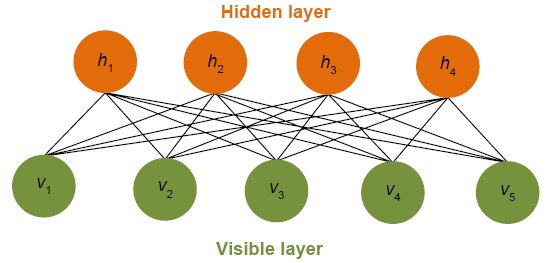
\includegraphics[scale=0.5]{chap3-img/RBM}
	\caption{ماشین بلتزمن محدود}
	\label{chap3-fig1}
\end{figure}

محدود بودن به طول بردار ثابت برای داده‌های ورودی و همچنین حالت باینری برای آن‌ها از مشکلات مدل
RBM
است که علی‌رغم قدرت بسیار بالای این مدل در تخمین توزیع داده‌های ورودی باعث گردیده در کاربردهای دنیای واقعی‌ آنچنان که باید مورد استفاده قرار نگیرد.
	
	\subsection{مدل شبکه‌‌ی عصبی خود رگرسیو تخمین‌زننده‌ی توزیع }
	\label{chap3sec2sub2}
	مدل
	NADE
	که از مدل
	RBM
	الهام گرفته شده است، یک روش احتمالاتی مولد بدون‌نظارت برای مدل‌سازی احتمال داده‌های گسسته در ابعاد بالا می‌‌باشد
	\cite{larochelle2011neural}.
	 در این روش نیز همانند مدل
	RBM
	طول بردار ورودی ثابت در نظر گرفته می‌‌شود، همچنین ورودی نیز ماند شبکه‌ی
	RBM
	محدود به حالت باینری می‌‌باشد
	\cite{larochelle2011neural}.
	
	 مشکل دیگر موجود در مدل
	RBM
	 مناسب نبودن این مدل برای تخمین احتمال مشترک در ابعاد بالا می‌باشد. این مشکل در مدل
	NADE 
	بدلیل استفاده از ایده‌ی شبکه‌های بیزین کاملا مشاهده‌پذیر\LTRfootnote{Fully Visible Bayesian Networks}
		(FVBN)
	\cite{dayan1996does}\cite{bengio1999modeling}
	برای محاسبه‌ی احتمال مرتفع گردیده است. در این شبکه‌ها برای محاسبه‌ی احتمال مشاهده‌ی یک بردار ورودی مانند
	$\textbf{V}$
	توسط مدل از رابطه‌ای مشابه رابطه
	\ref{chap3-eq4}
	استفاده می‌‌شود، که در آن
	$\textbf{V}_{parent(i)} = \textbf{V}_{<i}$
	اشاره به یک زیربردار دارد که شامل تمام ابعاد قبل از
	$i$امین 
بعد می‌‌باشد. به بیان دیگر در این شبکه‌ها قبل از ساختن مدل، برای داده‌های ورودی یک ترتیب فرضی‌ برای ابعاد آن در نظر گرفته می‌‌شود و سپس یک بردار جهت‌دار به مدل به عنوان ورودی داده می‌‌شود و
	$\textbf{V}_{<i}$
	 یک بردار جهت‌دار شامل تمام ابعاد تا قبل از
	$i$امین 
	بعد می‌‌باشد. با تعریف بیان شده می‌‌توان گفت که در این شبکه‌ها احتمال هر بعد از بردار ورودی مشروط به تمام ابعاد قبل از آن محاسبه می‌گردد. بنابراین اگر تمام
	$p(v_i|\textbf{V}_{parent(i)})$ها
	از نظر جبری قابل محاسبه باشند در نتیجه بدست آوردن مقدار
	$p(\textbf{V})$
	از نظر محاسباتی امکان پذیر می‌‌باشد
	\cite{larochelle2011neural}.
	\begin{align}
	\centering
	\label{chap3-eq4}
	p(\textbf{V}) = \prod_{i=1}^{D}(v_i|\textbf{V}_{parent(i)})
	\end{align}
	
	در مدل
	NADE
	نیز که از رابطه‌ی
	\ref{chap3-eq4}
	برای محاسبه‌ی احتمال یک بردار ورودی استفاده می‌شود، می‌‌توان احتمال داده‌های با ابعاد بالا را مشروط به تمام ابعادش محاسبه کرد. در شکل‌های
	\ref{chap3-fig2-1}
	و
	\ref{chap3-fig2-2}
	به ترتیب مدل‌های
	FVBN
	و
	NADE
	نشان داده شده‌اند. همان‌طور که بیان شد و در شکل
	\ref{chap3-fig2-2}
	نیز مشاهده می‌‌گردد در مدل
	NADE
	به طور مثال مقدار احتمال بعد سوم بردار ورودی که با
	$\hat{v_3}$
	نشان داده می‌‌شود از یک لایه‌ی پنهان بدست می‌‌آید که تنها وابسته به ابعاد قبل از
	$v_3$
	یعنی‌
	$v_2$
	و
	$v_1$
	در بردار ورودی می‌‌باشد
	\cite{larochelle2011neural}.

	\begin{figure}[!t]
		\centering
		\begin{subfigure}{0.4\textwidth}
			\centering
			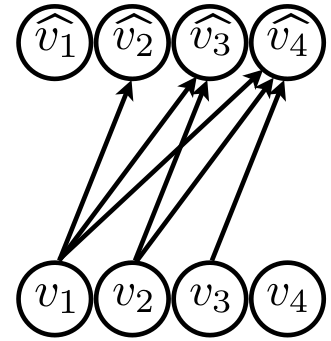
\includegraphics[scale=0.25]{chap3-img/FVSBN}
			\caption{مدل FVBN}
			\label{chap3-fig2-1}
		\end{subfigure}		
		\begin{subfigure}{0.4\textwidth}
			\centering
			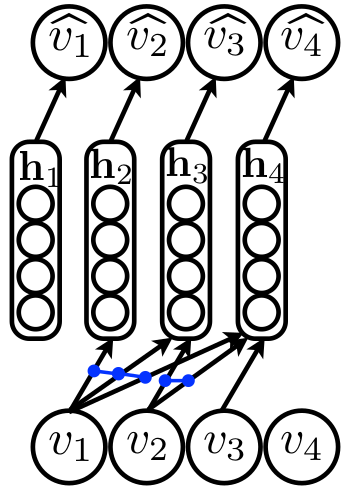
\includegraphics[scale=0.25]{chap3-img/NADE}
			\caption{مدل NADE}
			\label{chap3-fig2-2}
		\end{subfigure}
		\caption{مدل‌های FVBN و NADE}
		\label{chap3-fig2}
	\end{figure}


\section{روش‌های مدل‌سازی موضوعی}
\label{chap3sec3}
همان‌طور که پیش از این در بخش
\ref{chap2sec12}
بیان کردیم روش‌های مدل‌سازی موضوع به مدل‌هایی گفته می‌‌شود که یک چکیده از موضوعات موجود در یک سند یا مجمومه‌ای از اسناد را تشخیص داده و استخرج می‌‌کنند. این مدل‌ها را می‌‌توان در دو دسته‌ی کلی‌ شامل مدل‌های گرافی که بر پایه‌ی قوانین احتمالاتی و رابطه‌‌ی بیز می‌‌باشند و همچنین مدل‌های شبکه‌های عصبی تقسیم‌بندی کرد. در ادامه ضمن معرفی هر کدام از این کلاس‌ها با مهمترین مدل‌های موجود در این حوضه آشنا می‌‌گردیم.
	\subsection{مدل تکرار عبارت-معکوس تکرار سند}
	\label{chap3sec3sub1}
	 تاکنون محققین حوضه‌ی بازیابی اطلاعات پیشرفت‌های قابل توجهی‌ در زمینه‌ی مدل کردن مجموعه‌ی اسناد یا هر مجموعه‌ی گسسته‌ از داده‌ها داشته‌اند
	\cite{baeza1999modern}.
	در روش پایه که توسط پژوهشگران حوزه‌ی
	IR
	پیشنهاد گردیده و امروزه همچنان در مرورگر‌های اینترنتی مورد استفاده قرار می‌‌گیرد، هر سند متنی از یک مجموعه اسناد به یک بردار اعدد حقیقی‌ تبدیل می‌شود که شامل نسبت‌های تعداد تکرار کلمات مختلف می‌‌باشد.
	
	 در این روش که به آن تکرار عبارت-معکوس تکرار سند\LTRfootnote{Term Frequency-Inverse Document Frequency} 
	($tf-idf$) \cite{salton1986introduction}
	گفته می‌شود و در سال 1986 توسط
	Salton
	معرفی شد یک لغات‌نامه از تمام کلمات متمایز ساخته می‌‌شود، سپس برای هر سند در مجموعه‌ی اسناد تعداد رخداد تمام کلمات متمایز محاسبه می‌‌شود. پس از نرمال‌سازی مناسب (بیشتر در مقیاس لگاریتمی) مقادیر بدست آماده برای هر کلمه، هر مقدار بر معکوس تعداد سندهای شامل آن کلمه در کّل مجموعه‌ی اسناد تقسیم می‌‌گردد. مقادیر نهایی بدست آماده برای هر کلمه که به آن مقادیر
	$tf-idf$
	گفته می‌شود به صورت یک بردار ستونی در یک ماتریس جایگذاری می‌شوند. بنابراین در روش
	$tf-idf$
	یک مجموعه سند به ماتریسی
	$m \times n$
	تبدیل می‌شود که در آن
	$m$
	تعداد کلمات متمایز در مجموعه سند و
	$n$
	تعداد سندهای موجود در مجموعه سند می‌‌باشند.
	
	به عنوان مثال یک مجموعه اسناد که تنها از دو سند تشکیل شده است را در نظر بگیرید. اگر جدول تکرار کلمه‌ها برای هر سند مانند شکل
	\ref{chap3-fig3}
	باشد، آنگاه محاسبه‌ی
	$tf-idf$
	برای یک کلمه مانند
	$"this"$
	به صورت زیر می‌‌باشد:
\begin{flushleft}
$Document_1:\  tf("this",d_1) = \dfrac{1}{5} = 0.2 \qquad Document_2:\  tf("this",d_2) = \dfrac{1}{7} \approx 0.14$

$idf("this",D) = \log(\dfrac{2}{2}) = 0$

$Document_1:\  tfidf("this",d_1) = 0.2 \times 0 = 0 \qquad Document_2:\  tfidf("this",d_2) = 0.14 \times 0 = 0$
\end{flushleft}
صفر شدن مقدار 
$tf-idf$ 
برای 
$"this"$ 
نشان می‌‌دهد که این کلمه از آنجا که در تمام سند‌ها تکرار شده است بنابراین از اهمیت کمی‌ برخوردار می‌‌باشد.   
	\begin{figure}[b]
		\centering
		\begin{subfigure}{0.3\textwidth}
			\centering
			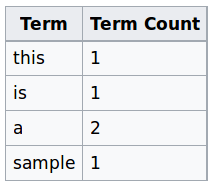
\includegraphics[scale=0.4]{chap3-img/tf-idf1}
			\caption{سند اول}
			\label{chap3-fig3-1}
		\end{subfigure}		
		\begin{subfigure}{0.3\textwidth}
			\centering
			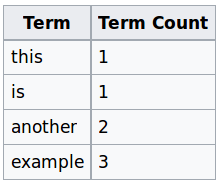
\includegraphics[scale=0.4]{chap3-img/tf-idf2}
			\caption{سند دوم}
			\label{chap3-fig3-2}
		\end{subfigure}
		\caption{جدول‌های تعداد تکرار کلمات برای یک مجموعه‌ی اسناد ۲ سندی}
		\label{chap3-fig3}
	\end{figure}
	
	\subsection{مدل فهرست‌سازی معنایی نهفته}
	\label{chap3sec3sub2}
	علی‌رغم ویژگی‌‌های مناسب مدل کاهش‌دهنده‌ی
	$tf-idf$
	مانند شناسایی مجموعه کلمه‌هایی که برای هر سند آن را از دیگر سند‌ها در یک مجموعه متمایز می‌‌کند، مشکلاتی مانند میزان کاهش ناچیز طول هر سند و همچنین در نظر نگرفتن خصوصیت آماری‌ در داخل هر سند از نقاط ضعف این روش می‌‌باشد. برای غلبه بر این مشکلات محققین حوزه‌ی
	IR
	چندین مدل کاهش بعد دیگر معرفی‌ کردند که مهمترین آن‌ها مدل فهرست کردن معنایی نهفته\LTRfootnote{Latent Semantic Indexing}
	(LSI)
	می‌باشد که توسط
	Deerwester \cite{deerwester1990indexing}
	 و همکاران در سال 1990 ارائه گردید.
	
	مدل
	LSI
	با استفاده از تجزیه مقدار منفرد\LTRfootnote{Singular Value Decomposition}
	 بر روی ماتریس خروجی از مدل
	$tf-idf$
	یک زیرفضای خطی\LTRfootnote{Linear Subspace}
	‌ در فضای ویژگی‌‌های مدل
	$tf-idf$
	شناسایی می‌‌کند. این روش منجر به کاهش و فشرده‌سازی قابل توجهی‌ در مجموعه‌های بزرگ می‌‌گردد. همچنین
	Deerwester
	و همکاران ادعا کردند که ویژگی‌‌های بدست آماده توسط مدل
	LSI
	که در حقیقت یک ترکیب خطی‌ از ویژگی‌‌های مدل
	$tf-idf$
	می‌باشند، توانایی تشخیص بعضی‌ از ویژگی‌‌های زبانی مانند مترادف و متضاد را دارند
	\cite{deerwester1990indexing}.
	
	\subsection{مدل فهرست‌سازی معنایی نهفته‌ی احتمالاتی}
	\label{chap3sec3sub3}
	برای اثبات ادعا‌های مطرح شده توسط مدل
	LSI (بخش \ref{chap3sec3sub2})
	و همچنین بررسی‌ نقاط ضعف و قدرت این مدل، روش فهرست‌سازی معنایی نهفته‌ی احتمالاتی\LTRfootnote{probabilistic Latent Semantic Indexing} (pLSI)
	 توسط 
	Hofmann \cite{hofmann1999probabilistic}
در سال 1999 معرفی شد. مدل 
	pLSI
	یک مدل مولد احتمالاتی می‌باشد که از آن به عنوان یک مدل موضوعی نیز یاد می‌شود
	\cite{blei2003latent}.
	 در روش 
	 pLSI
	 هر کلمه‌ی داخل هر سند به عنوان یک نمونه از یک مدل مخلوط مدل می‌شود
	 \cite{hofmann1999probabilistic}.
	  مؤلفه‌های این مدل مخلوط در واقع متغیرهای تصادفی چندجمله‌ای می‌باشند که می‌توان آن‌ها را به عنوان یک نمایش از موضوع‌های موجود در سند دانست. بنابراین هر کلمه از یک موضوع خاص تولید می‌‌شود و کلمه‌های مختلف در داخل یک سند ممکن است از موضوع‌های مختلفی‌ تولید شوند. در نتیجه هر سند به صورت لیستی از این توزیع‌های مخلوط نمایش داده می‌‌شود و در واقع هر سند به یک مجموعه‌ی از پیش تعیین شده از نظر تعداد از توزیع‌های احتمالاتی کاهش پیدا می‌کند.
	
	در شکل
	\ref{chap3-fig4}
	مدل
	pLSI
	را مشاهده می‌کنید‌. در شکل
	\ref{chap3-fig4}
	 مجموعه سند دارای
	M
	سند مختلف می‌‌باشد که هر کدام از آن‌ها دارای
	N
	کلمه‌ می‌‌باشند.همچنین در این شکل
	(\ref{chap3-fig4})، $w$
	نشان دهنده‌ي کلمه، و
	$z$
	نماد یک توزیع چندجمله‌ای از موضوع‌ها در یک سند مشخص می‌‌باشد. با توجه به شکل
	\ref{chap3-fig4}
	و توضیحات بیان شده، در مدل
	pLSI
	فرض بر آن است که یک سند مانند
	$d$
	و یک کلمه‌ مانند
	$w_n$
	در صورت داشتن یک موضوع مشاهده نشده مانند
	$z$
	همان‌طور که در رابطه
	\ref{chap3-eq5}
	مشاهده می‌‌شود دارای استقلال شرطی از یکدیگر می‌‌باشند.
	\begin{align}
	\centering
	\label{chap3-eq5}
		p(d,w_n) = p(d) \sum_{z} p(w_n|z)p(z|d)
	\end{align}
	همان‌طور که پیش از این در بخش
	\ref{chap2sec12}
	بیان شد، یک فرض اساسی‌ که مدل‌های موضوعی بر اساس آن ساخته می‌‌شوند در نظر گرفتن چند موضوع برای هر سند می‌‌باشد. مدل
	pLSI
	به عنوان یک مدل موضوعی این امکان را در رابطه‌ی
	\ref{chap3-eq5}
	برای یک سند مشخص مانند
	$d$
	با ترم
	$p(z|d)$
	در نظر می‌‌گیرد. توجه شود که در اینجا برچسب
	$d$
	یک برچسب ساختگی برای سند‌های مجموعه داده‌ی آموزش می‌‌باشد، در حقیقت
	$d$
	یک متغیر تصادفی چندجمله‌ای می‌‌باشد که مقادیر ممکن برای آن برابر با تعداد سند‌های موجود در مجموعه داده‌ی آموزش که مدل در آن
	$p(z|d)$
	را یاد می‌‌گیرد، می‌‌باشد. به همین دلیل مدل
	pLSI
	یک مدل مولد مناسب برای اسناد‌ نمی‌‌باشد، چرا که هیچ راهی‌ برای تقابل و تخصیص احتمال به موضوع‌هایی که آن‌ها را در داده‌های آموزش مشاهده 
	نکرده است در این مدل وجود ندارد
	\cite{blei2003latent}.
	
	مشکل دیگر مدل
	pLSI
	بدلیل استفاده از توزیع‌های احتمالی‌ موجود در داده‌های آموزش می‌‌باشد که باعث می‌‌شود پارامترهایی که باید توسط مدل تخمین زده شوند به صورت خطی با اندازه داده‌های آموزش رشد پیدا کنند
	\cite{blei2003latent}.
	\begin{figure}
		\centering
		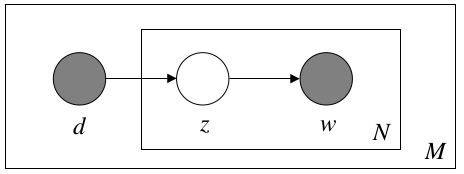
\includegraphics[scale=0.4]{chap3-img/pLSI}
		\caption{مدل فهرست‌ساری معنایی نهفته‌ی احتمالاتی \cite{blei2003latent}}
		\label{chap3-fig4}
	\end{figure}
	
	
	\subsection{مدل تخصیص دیریکله‌ی پنهان}
	\label{chap3sec3sub4}
	مدل تخصیص دیریکله‌ی پنهان 
\LTRfootnote{Latent Dirichlet Allocation}	(LDA)
	یک مدل احتمالاتی مولد گرافی می‌باشد که در سال 2003 توسط 
	Blei 
	و همکاران
	\cite{blei2003latent}
	معرفی شد و پس از آن به عنوان پایه و اساس مدل‌سازی موضوع در بخش روش‌های گرافی‌ قرار گرفت. مدل
	LDA
	 را می‌‌توان معروف‌ترین و مهم‌ترین روش مدل‌سازی موضوع در بخش مدل‌های گرافی‌ و مدل‌های بیزی دانست. تا به امروز روش‌های بسیاری از این مدل برای کاربرد‌های مختلف مشتق شده‌اند که در بخش‌های
	 \ref{chap3sec4sub1}
	 و
	 \ref{chap3sec4sub2}
	 دو مورد از آن‌ها را که به تشخیص همزمان موضوع و احساس از داده‌های متنی می‌‌پردازند را بررسی‌ می‌‌کنیم.
	 
	 
	 
	 در روش  
	LDA
	مانند دیگر روش‌های مدل‌سازی موضوع، هر سند متنی به صورت یک توزیع مخلوط بر روی موضوع‌های مختلف‌ که در آن هر موضوع به وسیله‌ی یک توزیع بر روی کلمه‌ها مشخص می‌‌شود در نظر گرفته می‌شود
	\cite{blei2003latent}.
	شکل
	\ref{chap3-fig5}
	مدل
	LDA
	استاندارد را نشان می‌‌دهد.	
	
همان‌طور که در بخش
\ref{chap3sec3sub3}
بیان شد مدل
pLSI
از مشکلاتی مانند بزرگ شدن فضای پارامترهای مساله به صورت خطی‌ با اندازه داده ‌های آموزش و همچنین عدم توانایی در تخصیص احتمال به موضوع‌ها و سند‌های از پیش دیده نشده رنج می‌‌برد. مدل
LDA
با در نظر گرفتن وزن‌های توزیع مخلوط موضوع‌ها به عنوان یک متغیر تصادفی پنهان، به جای یک مجموعه بزرگ از پارامترهای منحصر به فرد که 
مستقیما به داده‌های آموزش متصل باشند بر این دو مشکل غلبه کرده است.
	\begin{figure}[!t]
		\centering
		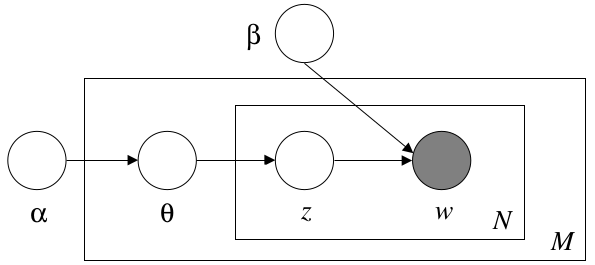
\includegraphics[scale=0.4]{chap3-img/LDA}
		\caption{مدل تخصیص دیریکله‌ی پنهان \cite{blei2003latent}}
		\label{chap3-fig5}
	\end{figure}

در مدل
LDA
که در شکل
\ref{chap3-fig5}
نشان داده شده است،
$\beta$
یک ماتریس دو بعدی احتمالاتی با اندازه
$k \times V$
 می‌‌باشد که در آن
$k$
برابر با تعداد موضوع‌ها و
$V$
برابر با اندازه لغت‌نامه‌ یا تعداد کلمات متمایز در متن می‌‌باشد. درایه‌های این ماتریس، احتمال حضور هر کلمه در هر موضوع را نشان می‌‌دهند. برای مثال
$\beta_{ij}$
نشان دهنده‌ی احتمال حضور کلمه‌ی
$j$ام
 در موضوع
$i$ام
 می‌باشد. همان‌طور که در بخش
\ref{chap2sec4}
در مورد مدل‌های گرافی توضیح داده شده در شکل
\ref{chap3-fig5}
پارامتر‌های
$\beta,\ \alpha,\ \theta ,\ z$
متغیر‌های پنهان می‌‌باشند و
$w$
تنها متغیر قابل مشاهده در مدل
LDA
می‌ باشد.

در مدل
LDA
پارامتر
$\alpha$
یک بردار
$k$
بعدی که
$k$
تعداد موضوع‌ها را نشان می‌دهد، می‌‌باشد.
$\alpha$
احتمال اولیه‌ی یک توزیع دیریکله می‌‌باشد که با نمونه گرفتن از آن با استفاده از رابطه‌ی
\ref{chap3-eq6}
به ازای هر سند بردار
$\theta$
که یک توزیع چندجمله‌ای می‌‌باشد و نشان دهنده‌ی توزیع موضوع‌ها در هر سند می‌‌باشد را بدست می‌‌آوریم. در رابطه‌ی
\ref{chap3-eq6}، $\Gamma$
تابع گاما می‌‌باشد که در بخش
\ref{chap2sec8}
آن را معرفی‌ کردیم.
\begin{align}
	\centering
	\label{chap3-eq6}
	p(\theta|\alpha) = \dfrac{\Gamma (\sum_{i=1}^{k} \alpha_i)}{\prod_{i=1}^{k} \Gamma(\alpha_i)} \theta_1^{\alpha_1 -1}\ ...\ \theta_k^{\alpha_k -1}
\end{align}

با داشتن
$\alpha$
و
$\beta$
توزیع مشترک پارامترهای
$\theta$، $\textbf{z}$
و
$\textbf{w}$
از رابطه‌ی
\ref{chap3-eq7}
بدست می‌‌آید. در رابطه‌ی
\ref{chap3-eq7}، $\theta$
یک توزیع چندجمله‌ا‌ی موضوعی، بردار
$\textbf{z}$
یک مجموعه
$N$تائی‌
 از موضوع‌ها که از
$\theta$
نمونه گرفته می‌‌شود و
$\textbf{w}$
یک مجموعه
$N$
تائی‌ از کلمه‌ها که مشروط به
$\beta$
و
$z$
نمونه گرفته می‌‌شود. در ادامه با انتگرال‌گیری روی
$\theta$
و سیگما روی
$z$
 احتمال حاشیه‌ای برای یک سند به فرم رابطه‌ی
 \ref{chap3-eq8}
  بدست می‌‌آید. و در نهایت با ضرب احتمال‌های حاشیه‌ای برای هر سند احتمال یک مجموعه سند به شکل رابطه‌‌ی
 \ref{chap3-eq9}
  بدست می‌‌آید.
\begin{align}
\centering
\label{chap3-eq7}
	p(\theta,\textbf{z},\textbf{w}|\alpha,\beta) = p(\theta|\alpha)\prod_{n=1}^{N}p(z_n|\theta)p(w_n|z_n,\beta)
\end{align}
\begin{align}
\centering
\label{chap3-eq8}
p(\textbf{w}|\alpha,\beta) = \int p(\theta|\alpha) \left( \prod_{n=1}^{N} \sum_{z_n}p(z_n|\theta)p(w_n|z_n,\beta) \right)   d\theta
\end{align}
\begin{align}
\centering
\label{chap3-eq9}
p(D|\alpha,\beta) =\prod_{d=1}^{M} \int p(\theta|\alpha) \left( \prod_{n=1}^{N} \sum_{z_n}p(z_n|\theta)p(w_n|z_n,\beta) \right)d\theta_d
\end{align}

برای استنتاج در مدل
LDA
نمی‌توان از روش‌های مستقیم استفاده کرد و به جای آن باید از روش‌های تقریبی مانند، تقریب لاپلاس\LTRfootnote{Laplace Approximation}،
 تقریب تغییراتی\LTRfootnote{Variational Approximation}
 ‌ و یا روش
MCMC
که در بخش
\ref{chap2sec6}
معرفی‌ شد استفاده کرد. در مدل معرفی‌ شده توسط آقای
Blei
همکاران 
\cite{blei2003latent}
در سال ۲۰۰۳ از روش تقریب تغییراتی‌ برای استنتاج در مدل
LDA
استفاده شده است. شکل
\ref{chap3-fig11}
خروجی مدل
LDA
برای چهار موضوع مختلف به همراه کلماتشان در یک متن نمونه را نشان می‌‌دهد.

	\begin{figure}[!t]
		\centering
		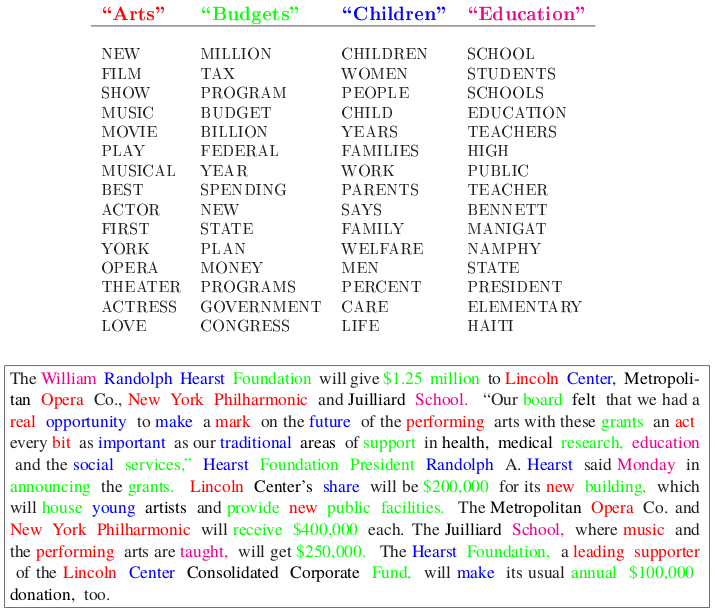
\includegraphics[scale=0.4]{chap3-img/LDAexample}
		\caption{نمونه خروجی مدل LDA برای چهار موضوع مختلف \cite{blei2003latent}}
		\label{chap3-fig11}
	\end{figure}



	\subsection{مدل Softmax تکرارشده}
	\label{chap3sec3sub5}
	
	مدل
	Softmax
	تکرارشده\footnote{Replicated Softmax}
	(RS)
	که در سال ۲۰۰۹ توسط
	Hinton
	و
	Salakhutdinov \cite{hinton2009replicated}
	معرفی‌ شد، اولین روش مدل‌سازی موضوع بر پایه‌ی شبکه‌های عصبی است.
	RS
	گسترش‌یافته‌ی مدل
	RBM
	می‌باشد که از آن برای تشخیص توزیع موضوع‌های مختلف در داده‌های متنی استفاده می‌‌شود. مدل
	RBM
	به دلیل محدودیت‌هایی مانند محدود بودن به بردار ورودی باینری و در نظر گرفتن طول ثابت برای وروی‌ها نمی‌‌تواند در تشخیص توزیع موضوع مورد استفاده قرار بگیرد، چرا که اولا کلمات باینری نیستند و دوما در یک مجموعه از داده‌های متنی طول اسناد با یکدیگر متفاوت می‌‌باشند
	\cite{hinton2009replicated}.
	
	در شکل
	\ref{chap3-fig6}
	مدل
	RS
	نشان داده شده است. همان‌طور که در شکل
	\ref{chap3-fig6}
	مشاهده می‌‌شود مدل
	RS
	مانند مدل
RBM
	دارای یک ساختار دو بخشی متشکل از یک لایه‌ی قابل مشاهده و یک لایه‌ی پنهان می‌‌باشد. در مدل
	RS
	نیز مانند مدل
	RBM
	یک تابع انرژی وابسته به سند ورودی و بردار پنهان آن به شکل رابطه‌ی
	\ref{chap3-eq10}
	تعریف می‌‌شود که ضمن کمینه کردن آن توزیع موضوع‌های مختلف در متن توسط مدل یاد گرفته می‌‌شود. احتمال مشاهده‌ی هر سند ورودی در این مدل به کمک رابطه‌ی
	\ref{chap3-eq11}
	محاسبه می‌‌گردد که در آن
	$Z$
	همانند مدل
	RBM
	تابع قسمت‌بندی می‌‌باشد و از رابطه
	\ref{chap3-eq12}
	بدست می‌‌آید.
	\begin{figure}[!t]
		\centering
		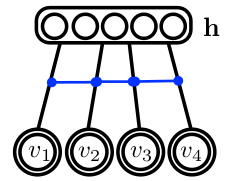
\includegraphics[scale=0.4]{chap3-img/RS}
		\caption{مدل Softmax تکرارشده \cite{hinton2009replicated}}
		\label{chap3-fig6}
	\end{figure}	
	\begin{align}
	\centering
	\label{chap3-eq10}
	E(\textbf{V},\textbf{h}) = -\sum_{j=1}^{F} \sum_{k=1}^{K} W_j^k h_j \hat{v}^k - \sum_{k=1}^K \hat{v}^k b^k -D\sum_{j=1}^F h_ja_j
	\end{align}
	\begin{align}
	\centering
	\label{chap3-eq11}
	p(\textbf{V}) = \dfrac{1}{Z}\sum_{h}exp(-E(\textbf{V},\textbf{h}))
	\end{align}	
	\begin{align}
	\centering
	\label{chap3-eq12}
	Z = \sum_{V}\sum_{h}exp(-E(\textbf{V},\textbf{h}))
	\end{align}
	در رابطه‌ی
	\ref{chap3-eq10}, D
	اندازه سند ورودی،
	$W$
	ماتریس وزن بین لایه‌ی قابل مشاهده و لایه‌ی پنهان،
	$\textbf{b}$
	و
	$\textbf{a}$
	به ترتیب بردار بایاس لایه‌های قابل مشاهده و پنهان می‌‌باشند. همچنین
	$\hat{v}^k$
	که آن را به صورت
	$\hat{v}^k = \sum_{i=1}^{D} v_i^k$
	 تعریف می‌‌کنیم برابر با تعداد
	$k$امین 
	کلمه‌ی لغت‌نامه می‌‌باشد. در مدل
		RS
	نیز مانند مدل
	RBM
	برای آموزش از الگوریتم
	CD
	که در بخش
	\ref{chap2sec7}
	معرفی شد استفاده می‌‌شود.
		 
	\subsection{مدل شبکه‌‌ی عصبی خود رگرسیو تخمین‌زننده‌ی توزیع سندی}
	\label{chap3sec3sub6}
مدل شبکه‌‌ی عصبی خود رگرسیو تخمین‌زننده‌ی توزیع سندی
\LTRfootnote{Document Neural Autoregressive Distribution Estimator}
(DocNADE)
که در شکل
\ref{chap3-fig7}
مشاهده می‌‌شود یک روش بدون‌نظارت برای مدل‌سازی موضوع بر پایه‌ی شبکه‌های عصبی می‌‌باشد. این مدل در سال ۲۰۱۲ توسط
Larochelle
و
Lauly \cite{larochelle2012neural}
با ترکیب مدل‌های
NADE
و
RS
معرفی‌ شد.

 بردار ورودی در این مدل بر خلاف مدل
NADE
که در آن بردار ورودی می‌‌بایست حتما باینری باشد، یک بردار چندجمله‌ای به شکل بردار ورودی در مدل
RS
می‌باشد. اما در این مدل مانند مدل
NADE
احتمال هر کلمه در داخل سند به شرط تمام کلمات قبل از آن بدست می‌‌آید
\cite{larochelle2012neural}.
 تفاوت دیگر مدل
DocNADE
با مدل
NADE
در نحوه‌ی بدست آوردن احتمال مشاهده‌ی هر کلمه به شرط کلمات قبل می‌‌باشد. در مدل
DocNADE
احتمال در لایه‌ی نهایی با استفاده از یک ساختار درختی محاسبه می‌‌گردد. در درخت مورد نظر که در شکل
\ref{chap3-fig7}
مشخص شده تمام کلمات در برگ‌های آن قرار می‌‌گیرند و هر مسیر از ریشه تا برگ برابر با احتمال مشاهده‌ی ‌کلمه‌ی متناظر با آن می‌‌باشد. استفاده از یک چنین ساختار درختی موجب می‌‌گردد تا بدست آوردن احتمال هر کلمه نسبت به اندازه لغت‌نامه مقداری لگاریتمی داشته باشد که در کاربرد‌های عملی‌ بسیار کارآمدتر از حالت مستقیم که خطی‌ می‌‌باشد است
\cite{larochelle2012neural}.

رابطه‌های
\ref{chap3-eq13}
و
\ref{chap3-eq14}
به ترتیب نحوه به دست آوردن مقادیر لایه‌ی پنهان و احتمال مشاهده‌ی هر کلمه به شرط تمام کلمات پیشین در مدل
DocNADE
 را نشان می‌‌دهند. در جدول
\ref{chap3-tb1}
نمونه‌ای از چهار موضوع یاد گرفته شده توسط مدل
DocNADE
به همراه ده کلمه‌ای‌ که در هر موضوع بیشترین احتمال را داشته‌اند مشاهده می‌شود.
\begin{align}
\centering
\textbf{h}_i(\textbf{v}_{<i}) = sigm(\textbf{c}+\sum_{k<i}\textbf{W}_{:,v_k})
\label{chap3-eq13}
\end{align}
\begin{align}
\centering
p(v_i=w|\textbf{v}_{<i}) = \frac{exp(b_w +\textbf{V}_{w,:}\textbf{h}_i(\textbf{v}_{<i})}{\sum_{w'}exp(b_{w'}+\textbf{V}_{w',:}\textbf{h}_i(\textbf{v}_{<i})}
\label{chap3-eq14}
\end{align}
  \begin{figure}[!t]
  	\centering
  	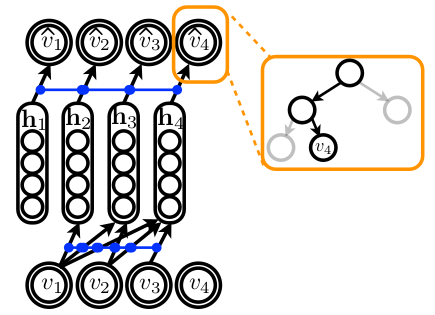
\includegraphics[scale=0.4]{chap3-img/DocNADE}
  	\caption{مدل شبکه‌‌ی عصبی خود رگرسیو تخمین‌زننده‌ی توزیع سندی \cite{larochelle2012neural}}
  	\label{chap3-fig7}
  \end{figure}

\section{مدل‌های مشترک موضوع و احساس}
تمام مدل‌های بررسی‌ شده در بخش‌های پیشین تنها توانایی تشخیص موضوع از داده‌های متنی را داشتند. گروه دیگری از مدل‌های موضوعی وجود دارند که به صورت همزمان به تشخیص موضوع‌ها و احساس همراه با هرکدام می‌‌پردازند. در بخش های
\ref{chap3sec4sub1}
و
\ref{chap3sec4sub2}
دو مدل موجود در این زمینه، که یکی‌ به تشخیص موضوع و احساس آن در سطح کلمه
(\ref{chap3sec4sub1})
 و یکی‌ در سطح جمله
(\ref{chap3sec4sub2})
  می‌‌پردازد را بررسی‌ می‌‌کنیم. همچنین در بخش
\ref{chap3sec4sub3}
  یک مدل با رویکردی نظارت شده که به تازگی برای تشخیص موضوع و احساس در داده‌های متنی پیشنهاد شده است را معرفی‌ می‌‌کنیم.
  \begin{table}[!b]
	\centering
	\begin{tabular}{|c|c|c|c|}
		\hline
		\multicolumn{4}{|c|}{چهار موضوع بادگرفته شده توسط DocNADE}\\
		\hline
		card 	 & shuttle 		& team 	   & christianity\\
		driver 	 & orbit 		& games    & god\\
		drivers  & lunar 		& seasons  & pgp\\ 
		bus		 & spacecraft 	& baseball & jesus\\ 
		video	 & nasa  		& players  & bible\\ 
		vga		 & space 		& game     & faith\\ 
		monitor  & launch 		& hockey   & muslim\\ 
		ibm   	 & saturn  		& play 	   & christ\\ 
		cards	 & billion		& teams    & atheist\\
		ram    	 & satellite	& sale     & christians\\
		\hline
	\end{tabular}
	\caption{نمومه‌ای از موضوع‌های یادگرفته شده توسط مدل DocNADE \cite{larochelle2012neural}}
	\label{chap3-tb1}
\end{table}

	\subsection{مدل یکی‌سازی احساس-موضوع}
	\label{chap3sec4sub2}
	
	پیدا کردن جنبه‌هایی از یک محصول که کاربران در بازبینی‌های آنلاین خود مورد ارزیابی قرار می‌‌دهند همواره کار مشکلی‌ بوده است. علاوه بر تشخیص موضوع‌ها و جنبه‌های موجود در یک بازبینی آنلاین، تشخیص احساس همراه با هر کدام نیز برای شرکت سازنده و افراد دیگری که به دنبال کسب اطلاعات در مورد یک محصول خاص می‌‌باشند، اهمیت دارد. مدل یکی‌سازی احساس-موضوع
\LTRfootnote{Aspect and Sentiment Unification Model}
	(ASUM)
	در سال ۲۰۱۱ برای تشخیص موضوع‌ها و احساس همراه با آن‌ها در بازبینی‌های آنلاین توسط
	Jo
	و
	Oh
	معرفی‌ شد
	\cite{jo2011aspect}.
	
	شکل
	\ref{chap3-fig9}
	مدل
	ASUM
	را نشان می‌‌دهد. این مدل همان‌طور که در شکل
	\ref{chap3-fig9}
	مشاهده می‌‌گردد گسترش یافته‌ی مدل
	LDA
	می‌باشد
	\cite{jo2011aspect}
	و در گروه مدل‌های احتمالاتی گرافی‌ مولد قرار می‌‌گیرد. در مدل
	LDA
	هر کلمه به صورت مجزا از یک موضوع نمونه گرفته می‌‌شود و فرض بر آن است که هر کلمه می‌‌تواند موضوع خود را داشته باشد، اما در مدل
	ASUM
	فرض بر آن است که هر جمله دارای یک موضوع می‌‌باشد و تمام کلمات یک جمله از یک موضوع نمونه گرفته می‌‌شوند
	\cite{jo2011aspect}.
	
در مدل
ASUM
ما برای هر سند یک توزیع چندجمله‌ای احساسی‌ و برای هر یک از احساس‌ها یک توزیع چندجمله‌ای موضوعی داریم. در حالت مولد پس از نمونه گرفتن از توزیع احساسی‌ و توزیع موضوعی متناسب با احساس انتخاب شده برای سند جاری، برای هر جمله یک احساس و یک موضوع نمونه گرفته ‌می‌‌شود و سپس تمام کلمات آن جمله از آن موضوع و احساس تولید می‌‌شوند
\cite{jo2011aspect}.

\begin{figure}[!t]
	\centering
	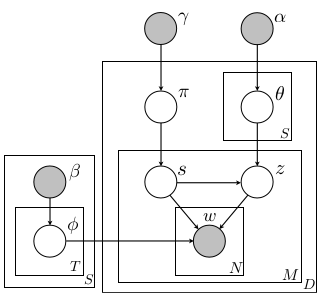
\includegraphics[scale=0.5]{chap3-img/ASUM}
	\caption{مدل یکی‌سازی احساس-موضوع \cite{jo2011aspect}}
	\label{chap3-fig9}
\end{figure}


	\subsection{مدل نظارت‌شده‌ی ضعیف تشخیص مشترک احساس-موضوع}
	\label{chap3sec4sub1}
مدل نظارت‌شده‌ی ضعیف تشخیص مشترک احساس/موضوع
(JST) \cite{lin2012weakly}
 که در شکل 
\ref{chap3-fig8}
مشاهده می‌‌شود در سال ۲۰۱۲ توسط
 Lin
 و همکاران معرفی‌ شد. مدل
 JST
  همانند 
 LDA
 یک مدل احتمالاتی مولد گرافی می‌‌باشد. در واقع
 JST
 گسترش یافته‌ی‌ مدل 
 LDA
 می‌‌باشد که علاوه بر تشخیص موضوع به تشخیص احساس از داده‌های متنی نیز می‌پردازد.  خاصیت نظارت‌شده‌ی ضعیف باعث می‌‌شود که در مقایسه با سایر مدل‌ها
 ، JST
  به راحتی‌ قابل انتقال به یک دامنه‌ی دیگر بدون کاهش محسوس در کارایی که در سایر مدل ها این اتفاق رخ می‌‌دهد باشد. از دیگر تفاوت‌های مدل
   JST
    با سایر مدل‌ها این است که تمام مدل‌های موجود به تشخیص احساس کلی‌ متن می‌پردازند، این در حالی‌ می‌‌باشد که
     JST
      به تشخیص احساس همراه با هر موضوع و احساس کلی‌ متن می‌‌پردازد که در مسائل پیش‌رو دید بهتری را به کاربر خواهد داد.
 
  برای مدل کردن احساس در 
 JST
 یک لایه بین سند و موضوع اضافه می‌شود. با وجود این، 
 JST
 یک مدل چهار لایه است که در آن اسناد با احساسات همراه هستند و احساسات با موضوع‌ها همراه هستند و در نهایت کلمات با هردو برچسب احساس و موضوع همراه هستند
 \cite{lin2012weakly}.
 
  فرض کنید که یک مجموعه سند در اختیار داریم که شامل
  D
   سند می‌‌باشد که به صورت  
  $C = \{d_1,\ ...,d_D\}$
   مشخص می‌‌شوند، هر سند موجود دنباله‌ای از  
  $N_d$
   کلمه می‌‌باشد که با  
   $d=\{w_1,\ ...,w_{N_d} \}$
    مشخص می‌‌شوند و هر کلمه در داخل سند یک مورد از 
    V
    کلمه‌ی مجزای واژگان می‌باشد که به صورت 
    $\{1,\ ...,V\}$
    شاخص‌گذاری شده‌اند. همچنین 
    S
    تعداد برچسب‌های احساس متمایز می‌‌باشد و 
    T
    برابر است با تعداد کلی‌ موضوع‌ها.
    
     روند تولید کلمه‌ی  
   $w_j$
    در سند 
    d
    تحت مدل 
    JST
    شامل سه‌ مرحله می‌‌شود. ابتدا یک برچسب احساس مثلا  
    $l$
    از  
    $\pi_d$
    که توزیع احتمالاتی احساس برای هر سند می‌‌باشد انتخاب شده، سپس با توجه به برچسب احساس انتخاب شده و مشروط به آن یک موضوع از توزیع موضوعی 
    $\theta_{d,l}$
     نمونه گرفته می‌شود. در نهایت با داشتن برچسب موضوع واحساس، ازتوزیع احتمالاتی مشروط به موضوع و احساس برای هر مجموعه سند یک کلمه تولید می‌شود. 
   	\begin{figure}[!h]
   		\centering
   		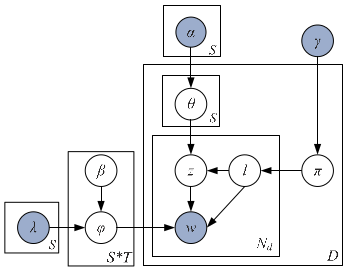
\includegraphics[scale=0.5]{chap3-img/JST}
   		\caption{مدل نظارت‌شده‌ی ضعیف تشخیص مشترک احساس/موضوع \cite{lin2012weakly}}
   		\label{chap3-fig8}
   	\end{figure}
    
     لازم به ذکر می‌‌باشد که در مدل 
     LDA
به ازای هر سند یک توزیع احتمالاتی برای موضوع‌ها وجود دارد، اما در مدل 
     JST
     به ازای هر برچسب احساس یک توزیع احتمالاتی برای موضوع‌ها در سند تعریف می‌شود. به طور مثال اگر سه‌ برچسب احساس مثبت، منفی‌ یا بی‌طرف در نظر گرفته شود، برای هر سند سه‌ توزیع احتمالاتی وجود خواهد داشت که هر کدام متناظر با یک احساس خواهند بود. تفاوت دیگری که بین مدل
LDA
       و
JST
می‌باشد از این قرار است که در
LDA
  به هنگام نمونه‌برداری از کلمه، این کار تنها مشروط به توزیع موضوعی برای مجموعه سند انجام می‌‌شود ولی‌ در
JST
    این نمونه برداری مشروط به هر دو توزیع موضوعی و احساسی‌ انجام می‌‌شود
    \cite{lin2012weakly}.
    در شکل
    \ref{chap3-fig12}
    می‌ توان خروجی مدل
    JST
    برای دو احساس مثبت 
    \ref{chap3-fig12-1}
    و منفی
    \ref{chap3-fig12-2}
    ‌  به همراه دو موضوع برای هر احساس و همچنین پانزده کلمه‌ای که بیشترین احتمال در هر موضوع داشتند را مشاهده می‌‌کنید.
    
	\begin{figure}[!b]
		\centering
		\begin{subfigure}{0.4\textwidth}
			\centering
			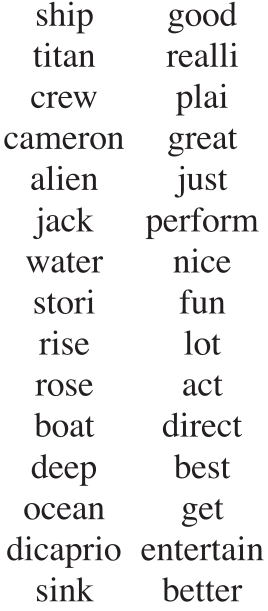
\includegraphics[scale=0.2]{chap3-img/JSTexamplep}
			\caption{نمونه خروجی مدل JST برای احساس مثبت}
			\label{chap3-fig12-1}
		\end{subfigure}		
		\begin{subfigure}{0.4\textwidth}
			\centering
			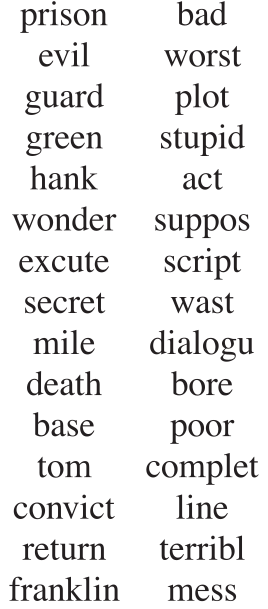
\includegraphics[scale=0.2]{chap3-img/JSTexamplen}
			\caption{نمونه خروجی مدل JST برای احساس منفی}
			\label{chap3-fig12-2}
		\end{subfigure}
		\caption{خروجی مدل JST برای دو احساس مثبت و منفی‌ و دو موضوع برای هر احساس و پانزده کلمه در هر موضوع \cite{lin2012weakly}}
		\label{chap3-fig12}
	\end{figure}

\subsection{مدل نظارت‌شده‌ی مشترک موضوع و احساس}
\label{chap3sec4sub3}
مدل نظارت‌شده‌ی مشترک موضوع و احساس
(SJASM)\footnote{Supervised Joint Aspect and Sentiment Model}
که در شکل
\ref{chap3-fig13}
 نشان داده شده است در سال ۲۰۱۷ توسط 
Hai
و همکاران معرفی‌ شد
\cite{7855825}. 
SJASM
یک رویکرد مولد احتمالی است که مانند مدل‌های 
ASUM
و 
JST
بر پایه‌ی روش 
LDA
است و در دسته‌ی روش‌های بیزی قرار می‌گیرد. SJASM با اضافه کردن چندین لایه و تغییر در ساختار مدل 
LDA
از برای تشخیص همزمان موضوع و احساس در داده‌های متنی مورد استفاده قرار می‌گیرد
\cite{7855825}.

در مدل 
SJASM
هر سند تولید شده توسط کاربران به صورت جفت کلمه‌های موضوع و احساس نمایش داده می‌شود. SJASM با استفاده از این جفت کلمه‌ها به مدل‌سازی مشترک موضوع و احساس در داده‌های متنی می‌پردازد
\cite{7855825}.
‌
	\begin{figure}[!t]
		\centering
		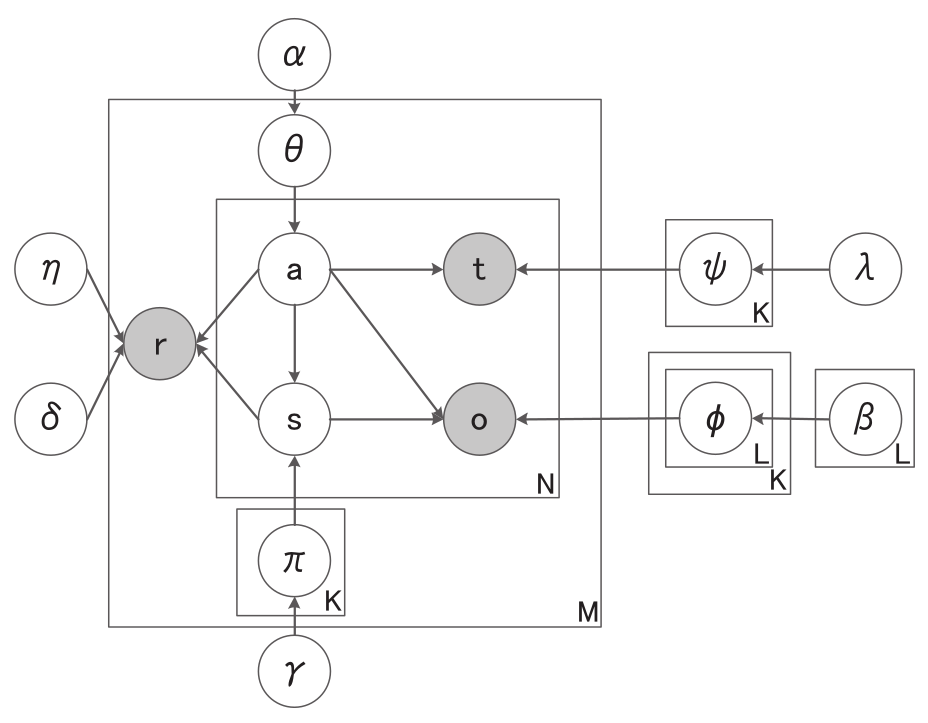
\includegraphics[scale=0.25]{chap3-img/SJASM}
		\caption{مدل نظارت‌شده‌ی مشترک موضوع و احساس \cite{7855825}}
		\label{chap3-fig13}
	\end{figure}


	
\section{مدل‌های چند حالته}
	مدل‌های چندحالته 
	\LTRfootnote{Multimodal}
	دسته‌ای از مدل‌های موضوعی می‌‌باشند که داده‌ی ورودی در آن‌ها ترکیبی‌ از چند حالت مختلف داده می‌‌باشد. در تمام مدل‌های معرفی‌ شده تا این قسمت از پژوهش، داده‌ی ورودی تنها اسناد متنی بودند یا به عبارت دیگر تنها یک حالت از داده به عنوان ورودی به مدل وارد می‌‌شود، اما مدل‌های چندحالته مانند آنچه که در بخش
	\ref{chap3sec5sub1}
	معرفی‌ می‌‌شود بر روی ترکیب همزمان دو یا چند حالت مختلف از داده مثلا تصویر و متن همراه با آن عمل می‌‌کنند.

	
	
	\subsection{مدل نظارت‌شده‌ی شبکه‌‌ی عصبی خود رگرسیو تخمین‌زننده‌ی توزیع سندی}
	\label{chap3sec5sub1}
	مدل نظارت‌شده‌ی شبکه‌‌ی عصبی خود رگرسیو تخمین‌زننده‌ی توزیع سندی\LTRfootnote{Supervised Document Neural Autoregressive Distribution Estimator}
	(SupDocNADE)
	 که در شکل 
	\ref{chap3-fig10}
	مشاهده می‌شود، در سال ۲۰۱۴ توسط
	Zheng
	و همکاران
	\cite{zheng2014topic}
	معرفی‌ شد. این مدل گسترش یافته‌ی مدل
	DocNADE
	می‌ باشد که در بخش
	\ref{chap3sec3sub6}
	معرفی‌ شد
	\cite{zheng2014topic}.
	 در مدل
	SupDocNADE
	داده‌های ورودی تنها اسناد متنی نمی‌‌باشند. ورودی در این مدل تصاویر به همراه توضیح کوتاهی‌ در مورد هر تصویر می‌‌باشد که مدل ترکیب این دو 
	نوع داده در کنار یکدیگر را یاد می‌‌گیرد. در این مدل ابتدا هر تصویر با استفاده الگوریتم‌های موجود در حوزه‌ی پردازش تصویر تغییر یافته و به یک سند متنی تبدیل شده و به توضیح مربوط به آن متصل می‌شود و به عنوان بردار ورودی به مدل وارد می‌‌شود
	\cite{zheng2014topic}.
	 تفاوت دیگر این مدل با مدل
	DocNADE
	اضافه کردن یک ساختار بر بایه‌ی شبکه‌ی عصبی در کنار قسمت‌های موجود می‌‌باشد که با استفاده از ویژگی‌‌های یاد گرفته شده از ترکیب هر تصویر و متن مربوط به آن عمل طبقه‌بندی را انجام می‌‌دهد
\cite{zheng2014topic}.
	
	\begin{figure}[!b]
		\centering
		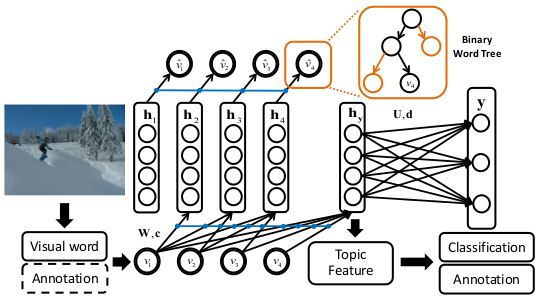
\includegraphics[scale=0.6]{chap3-img/SupDocNADE}
		\caption{مدل نظارت‌شده‌ی شبکه‌‌ی عصبی خود رگرسیو تخمین‌زننده‌ی توزیع سندی \cite{zheng2014topic}}
		\label{chap3-fig10}
	\end{figure}

\section{نتیجه‌گیری}
در این بخش پژوهش‌های پیشین در زمینه‌ی تخمین توزیع، مدل‌سازی موضوع، مدل‌سازی احساس‌-موضوع به صورت مشترک و همچنین مدل‌سازی داده‌های چندوحهی مورد بررسی‌ قرار گرفت. ساختار‌های بررسی‌ شده در این بخش در دو دسته‌ی مدل‌های شبکه‌های عصبی و مدل‌های گرافی‌ بیزین قرار می‌‌گیرند. در این پژوهش با ایده‌
گرفتن از ساختار‌های گرافی بیزین و استفاده از مدل‌های شبکه‌های عصبی هدف ساخت مدلی‌ برای شبیه‌سازی مشترک احساس و موضوع در داده‌های متنی می‌‌باشد. در بخش بعدی کلیات نظری مدل پیشنهادی در این پایان‌‌نامه و روابط و ساختار آن به صورت دقیق معرفی‌ و بررسی‌ می‌‌شوند.
 